\chapter{Compensation and Restitution of Post-Stroke Movement Patterns}
\label{cha:armeospring}

In this chapter, I present my study on the armeospring kinematics data.

\section{ArmeoSpring Overview}
\label{sec:overview}

The ArmeoSpring is a rehabilitation exoskeleton, designed for the purpose of ``functional arm and hand therapy''.\footnote{https://www.hocoma.com/usa/us/products/armeo/armeospring/} The device is based on research and development of David Reinkensmyer at the University of California, Irvine (UCI) and at the Rehabilitation Institute of Chicago (RIC). Shown in figure \ref{fig:armeo}, the exoskeleton has 7 degrees of freedom (DoF), summarized in table \ref{tab:devicedof}. It is attached to the arm by two or three velcro straps. The exoskeleton has two springs equipped, at the upper arm and forearm respectively. The springs can be adjusted to compensate the gravity force of the arm. The lengths of the exoskeleton are adjustable, as well as the strength of the springs. There are no motors at any joints, as a result, the user has to move actively to control the exoskeleton. The user's trunk is mildly constrained by the velcro strap at the upper arm. 

\begin{figure}
	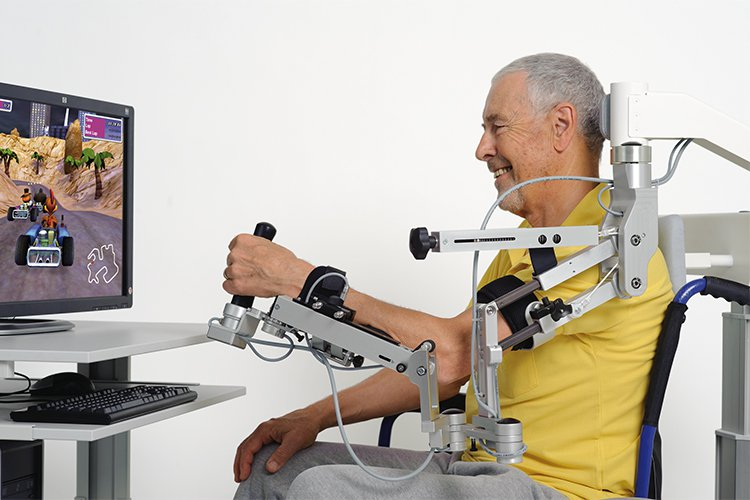
\includegraphics[width=0.5\textwidth]{armeo}
	\centering
	\caption{ArmeoSpring exoskeleton}
	\label{fig:armeo}
\end{figure}

\begin{table}
	\begin{tabular}{c c c c}
	\hline
	Joint No. & Joint Name & Anatomical Counterpart & Direction \\
	\hline
	1(1) & Inner Shoulder Angle & Shoulder Horizontal Ab-/Adduction & Left/Right \\
	1(2) & Outer Shoulder Angle & Shoulder Horizontal Ab-/Adduction & Left/Right \\
	2 & Upper Arm Angle & Shoulder Flex-/Extension & Up/Down \\
	3 & Elbow Angle & - & Left/Right \\
	4 & Forearm Angle & - & Up/Down \\
	5 & Pro-/Supination Angle & Pro-/Supination & - \\ 
	6 & Flex-/Extension Angle & Wrist Flex-/Extension & - \\
	\hline
	\end{tabular}
	\caption{Degrees of freedom of ArmeoSpring exoskeleton.}
	\label{tab:devicedof}
\end{table}

The device records all joint angles (that is, the joints of the exoskeleton), and calculates the end effector location through a forward kinematics model of the exoskeleton. The end effector location then is used to control a cursor on a screen, often displayed vertically in front of the user. The stick at the end point is equipped with a force sensor. During a training session, the user plays several 2D or 3D games, and after a certain game, the user is often presented with performance feedbacks of that game. Most of the games have difficulty settings that the physical therapist can change at the beginning of a training session.

The ArmeoSpring claims to be the most widely used arm and hand rehabilitation exoskeleton. The lack of motors enables self-initiated movement therapy. The device records all joint angles and end effector trajectories, as long as task-specific variables, which can be used to provide assessments and document patient progress.

\section{Data Collection: Control Group}
\label{datacontrol}

We recruited 11 young (age 23 $\pm$ 2) healthy subjects (7 males) to play the games which are designed for rehabilitation.

\subsection{Ladybug pointing test}

The ladybug pointing test (see figure \ref{fig:ladybug}) is a 2D game in which the user tries to catch ladybugs that appear one by one pseudo randomly. The game is 2D, so the direction that is perpendicular to the screen is ignored. To catch the ladybug, the user simply moves the cursor to its location. After a ladybug is caught, or a certain amount of time if not caught, the ladybug disappears and the next ladybug appears somewhere else. We chose this game as a test of performance because we know the beginning and end of each movement, namely from the current ladybug to the next.

\begin{figure}
	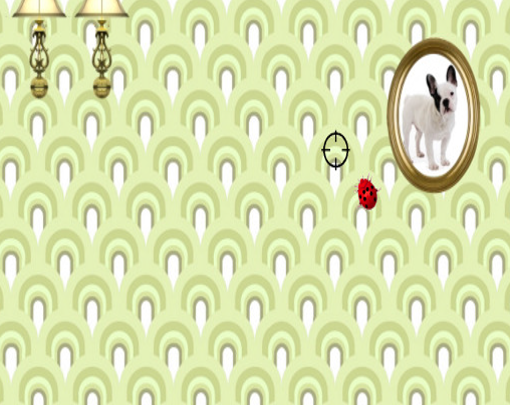
\includegraphics[width=0.5\textwidth]{ladybug}
	\centering
	\caption{Ladybug pointing test}
	\label{fig:ladybug}
\end{figure}

This pointing test is put at the beginning and the end of each training session. For subjects in control group, each session lasts about 20 minutes. There are 2 training sessions, one in the morning, the other in the afternoon, for 5 consecutive days. As a result, each subject has 10 sessions, 20 ladybug pointing tests. 

For control group, all games are set to be the most difficult level. Specifically, the ladybug pointing test for control group is set at level 4. There are 48 ladybugs in total. Though the locations of ladybugs seem to be random, they are actually appearing in a specific sequence at specific locations. In this case, all ladybugs appear on a 6*8 grid, with the sequence shown in \ref{fig:48order}.

As a result, the data consists movements that have various distances, various directions.

\section{Data Acquisition: Post-Stroke Group}

Data from post-stroke individuals is collected automatically when participants use ArmeoSpring under guidance from physical therapists. As a result, we have no control over the games difficulties and the arm length/ gravity compensation settings. However, all participants have similar schedules with the control group: there are 2 training sessions in a day, for 4 weeks, weekends excluded. As a result, each participant has 40 sessions, 80 ladybug pointing tests.

Now we have data from 41 post-stroke individuals; gender and affected side are balanced, shown in table \ref{tab:demog}. 